%!TEX root = ../thesis.tex

% TODO:
% 1. Improve quality.
% 2. Make sure we have a reference for everything. (e.g. add einstein paper)
% 3. Finish the "organized" part at the end.
% 4. Improve quality of Figure 1.
% 5. Maybe add that this is the basic for a project where new physics should
%    be found like e.g. NS eq. of state blabla.

\section{Introduction}
% Introduction to the general topic of GW
In 1916, Einstein predicted the existence of gravitational waves (GW). Nearly
100 years later, on September 14, 2015, the first detection of a gravitational
wave\cite{PhysRevLett.116.061102}, emitted by two merging black holes, confirmed
his prediction. This detection marked the beginning of the GW astronomy era.
Until then, it was also the last missing extrasolar messenger needed for 
full-scale multi-messenger physics.
\cite{Branchesi_2016} 

% Multi-Messenger physics: Importance of latency
Because multi-messenger physics utilizes different messengers to observe the 
same transient, it is of paramount interest to minimize the latency between 
the detector measuring the GW and its reported detection. This allows for
fast follow-up observations of the other messengers.

% Descibe the current situation: We have several detectors. The measurement is
% noisy.
When analyzing the \textit{strain} $h(t)$ measured by the detector, the
fundamental assumption is that it is made up by the GW \textit{signal} $s(t)$
and \textit{noise} $n(t)$ whereas

\begin{equation}
  h(t) = n(t) + s(t)
\end{equation}

Analyzing $h(t)$ about the possible occurence of $s(t)$ is currently done by
using an approach called matched filtering. Matched filtering works by 
convoluting precalculated models of expected signals, so called templates, with
the measured data generating a signal-to-noise (SNR) time series. Because the
parameters of the expected signals are not known in advance, the template bank
spans a large astronomical parameter space.
Using a SNR threshold, we can extract \textit{triggers} marking possible GW 
signals. Clustering together close triggers leads to a \textit{candidate event}.

Convoluting the measured data with the whole template bank is computationally
expensive, which in turn leads to a high latency between data aggregation and
the reported detection. This motivates the search for methods which are less
computationally expensive and thus provide a low-latency detection algorithm.

\begin{figure}[ht]
  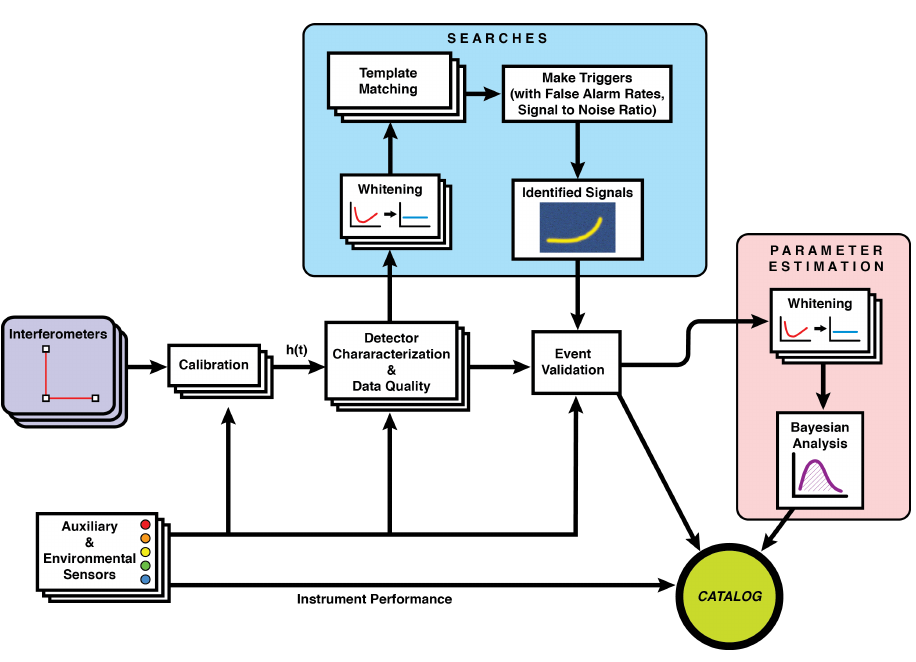
\includegraphics[width=0.95\textwidth]{img/1_introduction/data_processing.png}
  \caption{A simplified schematic summarizing the main steps in LIGO-Virgo data
           processing, from the output of the data to the results reported in a
           catalog of transient events.}
  \label{fig:1_data_processing}
  \centering
\end{figure}

In \autoref{fig:1_data_processing}, taken from \cite{2020CQGra..37e5002A},
we can see a simplified schematic summarizing the main steps in LIGO-Virgo data
processing. The detectors are highly sensitive which makes them prone to
different noise sources. One observed phenomenon are so called glitches which
can mimic true transient astrophysical signals \cite{2020CQGra..37e5002A}.
After a quality control, the data is being searched for GW signals and in case
a signal is found, called an candidate event, the parameters are being estimated.

Each candidate event gets a statistical significance assigned, which is given by the 
false-alarm rate (FAR) of the search. The FAR is basically telling us how many false positives
occured over the duration of the analyzed data. To count the amount of
false positives, we use the ranking statistic, given by the maximal SNR
of the considered candidate event, as the threshold. Current low-latency searches
do not distribute any event candidates with a FAR greated than 1 per month.
\cite{PhysRevD.98.024050}

In their pioneering works, \citeauthor{PhysRevD.97.044039} \cite{PhysRevD.97.044039}
and \citeauthor{PhysRevLett.120.141103} \cite{PhysRevLett.120.141103} showed
that convolutional neural networks (CNN) can be used to distinguish between
pure noise and noise containing a GW signal. Both works use a classical binary
classification framework where they utilize the \textit{false alarm probability}
(FAP) to compare their results to matched filtering. Applying matched filtering
on fixed sized samples to compute the FAP and using it to compare the two
approaches is problematic because the matched filtering approach used in the 
LIGO-Virgo data processing pipeline acts on a time series of arbitrary length
resp. on a continous data stream. \cite{PhysRevD.100.063015}

In this thesis, we will explore a similar deep learning (DL) approach to search,
for simulated GW signals in simulated white gaussian noise. While training a 
neural network (NN) is also rather computationally expensive, the evaulation of
a trained NN can be done in a fraction of a second. Furthermore future 
detections can easily be incorporated leading to an improved neural network.

This thesis is organized as follows. In Section 2 we first establish the data
used for our DL approach, so we know what we actually work with. In section 3 
we will describe the actual DL approach. In section 4, we present the results.
In section 5 we discuss possibilities for future work.

TODO: 
\begin{itemize}
  \item Figure 1: Better quality needed
  \item Text: Quality control
  \item Do I need to add a paragraph about the "openness" of the thesis?
  \item Do I need to comment about the generalilty of the code?
  \item "This thessi is the basis of a project"?
\end{itemize}



